\documentclass[a4paper,11pt]{article}

\usepackage[svgnames]{xcolor}
\usepackage{a4wide}
\usepackage{tikz}
\usetikzlibrary{arrows,pgfplots.groupplots}
\usepackage{pgfplots}
\pgfplotsset{compat=1.3}
\usepackage[detect-family]{siunitx}
\usepackage[eulergreek]{sansmath}
\sisetup{text-sf=\sansmath}
\usepackage{relsize}

\pagestyle{empty}

\begin{document}
% Based on station-layout.tex from Fokkema 2013.

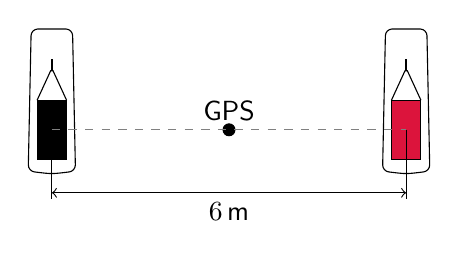
\begin{tikzpicture}
    [ font=\sffamily, x=.75cm, y=.75cm,
      hisparc/.style={draw},
    ]
    \foreach \col / \sx / \sy / \angle in {black/-3/0/180, Crimson/3/0/180} {
        \begin{scope}[hisparc, shift={(\sx,\sy)}, rotate=\angle]
            \draw[rounded corners=2.25pt]
                (-.4, .7) .. controls (0, .75) ..  (.4, .7) -- 
                (.35, -1.7) ..  controls(0, -1.72) ..  (-.35, -1.7) --
                cycle;
            \draw[fill=\col] (-.25, .5) rectangle (.25, -.5);
            \draw (-.25, -.5) -- (-.02, -1) --(.02, -1) -- (.25, -.5);
            \fill (-.02, -1) rectangle (.02, -1.2);
        \end{scope}
    }
    \draw[fill] (0, 0) circle (.10) node [above] {GPS};
%    \node[color=gray] at (-3.75, .75) {\Large 1};
%    \node[color=gray] at (2.25, .75) {\Large 2};

    \coordinate (A) at (-3, 0);
    \coordinate (B) at (3, 0);
    \coordinate (A') at ($ (A)!.8cm!-90:(B) $);
    \coordinate (B') at ($ (B)!.8cm!90:(A) $);
    \draw (A) -- ($ (A)!1.1!(A') $);
    \draw (B) -- ($ (B)!1.1!(B') $);
    \draw[<->] (A') -- (B') node [midway, below] {\SI{6}{\meter}};

    \coordinate (E) at (0, 0);

    \draw[dashed,gray] (A) -- (B);
\end{tikzpicture}

\end{document}
